\documentclass{BeamerTemplate}
\title{Module 3 - Quelques lois de probabilité discrètes}
\subtitle{STT-1000 Probabilités et statistique}
\date{\today}
\usepackage{adjustbox}


\begin{document}
\AtBeginSection{\frame{\sectionpage}}

\begin{frame}
\titlepage
\end{frame}

%-------------------------------------------------------------------------------------------------------------------------------------


\section{Introduction}

\begin{frame}{Contexte}

Il existe plusieurs lois discrètes bien connues, ayant même des noms pour les identifier, et pour lesquelles on connaît bien le comportement et les caractéristiques. 

\vspace{0.2in}
Plusieurs de ces lois sont reliées au résultats d'expériences aléatoires simples, par exemple une expérience qui peut résulter en un succès ou un échec. \\
Ex. On lance une pièce de monnaie. On déclare un succès si pile et échec si face.

\vspace{0.2in}
On verra cinq de ces lois dans le cours. 



\end{frame}


\begin{frame}[t]{Quelques résultats utiles pour les preuves}



\begin{itemize}
 \item {\bf Théorème du binôme (rappel):} 
 $$\sum\limits_{i=0}^n{n\choose i}x^iy^{n-i}= (x+y)^n$$
 \item {\bf Séries géométriques:} 
 $$ \sum_{i=0}^n p^i =  \frac{1-p^{n+1}}{1-p}$$
 $$ \sum_{i=0}^{\infty} p^i = 1+p+p^2+\cdots=\frac{1}{1-p} \; \; \; \alerter{ \mbox{ si } |p|<1}$$
  \item {\bf Expansion de $e^x$:} $$e^x=1+x+\frac{x^2}{2!}+\frac{3^3}{3!}+\cdots=\sum\limits_{i=0}^\infty\frac{x^i}{i!}$$
\end{itemize}
\end{frame}


\begin{frame}[t]{Un concept important - v.a. indépendantes}


Dans ce module et le suivant, on parlera à quelques reprises de \alerter{variables aléatoires indépendantes}. Ce concept sera formellement défini plus tard.

\vspace{0.2cm}
Pour l'instant, on se limite à cette définition: \alerter{deux variables aléatoires sont indépendantes si connaître la valeur de l'une des variables aléatoires ne nous renseigne en rien sur la valeur de la deuxième variable aléatoire. }

\vspace{0.1cm}
Si $X$ et $Y$ sont indépendants, nous notons $X \perp Y$.

Une propriété utile qui découle de l'indépendance de $X$ et $Y$ est 

$V(X+Y) = V(X) + V(Y).$

\begin{Boite}{Exemple}
{\small 
Je lance un dé et une pièce de monnaie. Soit $X$ qui est le résultat du dé et $Y$ qui prend la valeur $0$ si la pièce de monnaie tombe sur "pile" ou $1$ si la pièce de monnaie tombe sur "face. Alors, $X$ et $Y$ sont des variables aléatoires indépendantes. 
}
\end{Boite}

    
\end{frame}

\section{Loi de Bernoulli}

\begin{frame}[t]{Loi de Bernoulli}
Soit $X$ une variable aléatoire, telle que $X=1$ si l'expérience est un succès et $X=0$ si l'expérience est un échec. Nous associons une probabilité $p$ au succès et $1-p$ à l'échec. 

\bigskip
On dit que $X$ suit une loi de Bernoulli avec
probabilité $p$, ce qu'on dénote 
$$X\sim \mbox{Bernoulli}(p).$$

La fonction de probabilité de la loi
de Bernoulli$(p)$ est
$$
p(x)=\left\{\begin{array}{ll}
p, & x=1\\
1-p, & x=0\\
0, & \text{sinon.}
\end{array}\right.
$$

\end{frame}

\begin{frame}[t]{Loi de Bernoulli}

\textbf{Espérance}:

\vspace{2cm}

\textbf{Variance}:



\end{frame}

\section{Loi binomiale}

\begin{frame}[t]{Loi binomiale}
On suppose $Y_1,\hdots,Y_n$ des variables aléatoires indépendantes de même loi Bernoulli, i.e. $Y_i\sim \text{Bernoulli}(p)$, pour tout $i = 1,\hdots,n$.

\medskip 

On définit la variable aléatoire $X$ comme étant le nombre total de succès parmi $Y_1,\hdots,Y_n$. On peut écrire $$X=\sum_{i=1}^nY_i$$

\medskip
On dit que $X$ suit une loi binomiale avec paramètres $n$ et $p$, ce qu'on dénote
$$X\sim \mbox{Binomiale}(n,p).$$
\end{frame}

\begin{frame}{Loi binomiale}

{\small 

On veut $p(x) = P(X = x) = P(\mbox{observer $x$ succès}).$

\vspace{0.1 in}
Nous cherchons la probabilité d'avoir $x$ succès, et donc $n-x$ échecs. Puisque les essais sont indépendants, la probabilité de chacun des résultats avec $x$ succès et $n-x$ échec est 

$$ p^x (1-p)^{n-x}$$

Il faut prendre en compte le nombre de façons d'avoir $x$ succès parmi $n$ essais.

$$\displaystyle \binom{n}{x}$$



Donc, si $X\sim$Binomiale$(n,p)$, alors
$$p(x)=\left\{\begin{array}{ll}
{n\choose x}p^x(1-p)^{n-x}, & x=0,1,\ldots,n,\\
0, & \text{sinon}.
\end{array}\right.$$

}

\end{frame}


\begin{frame}{Loi binomiale}

Vérifiez que $p(x)$ donnée plus haut est bien une fonction de probabilité de masse.


\end{frame}


\begin{frame}{Loi binomiale}

\vspace{-0.1 in}

\begin{figure}[ht]
\begin{minipage}[b]{0.45\linewidth}
\centering
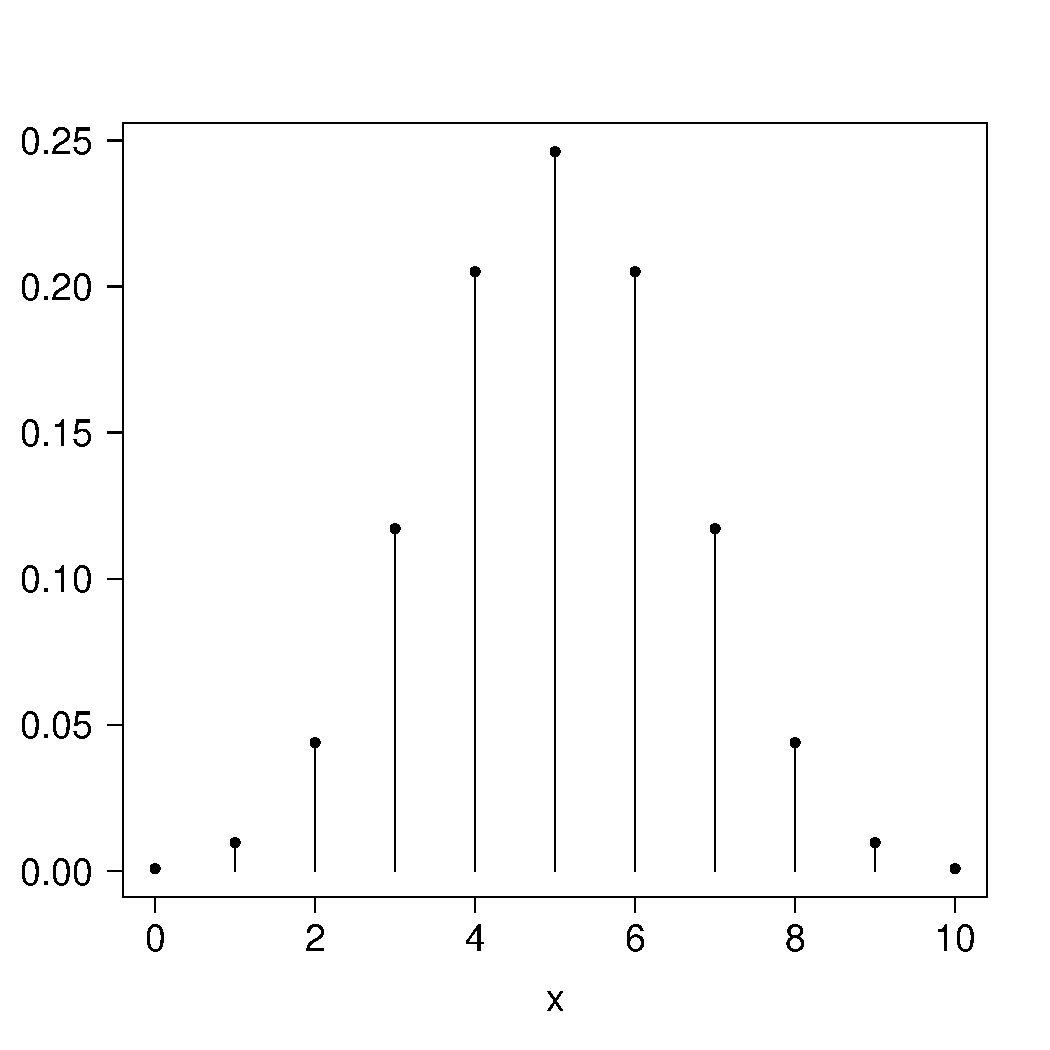
\includegraphics[scale = 0.2]{Binom1.pdf}\\
{\small Binomiale(n=10,p=0.5)}
\end{minipage}
\hspace{0.5cm}
\begin{minipage}[b]{0.45\linewidth}
\centering
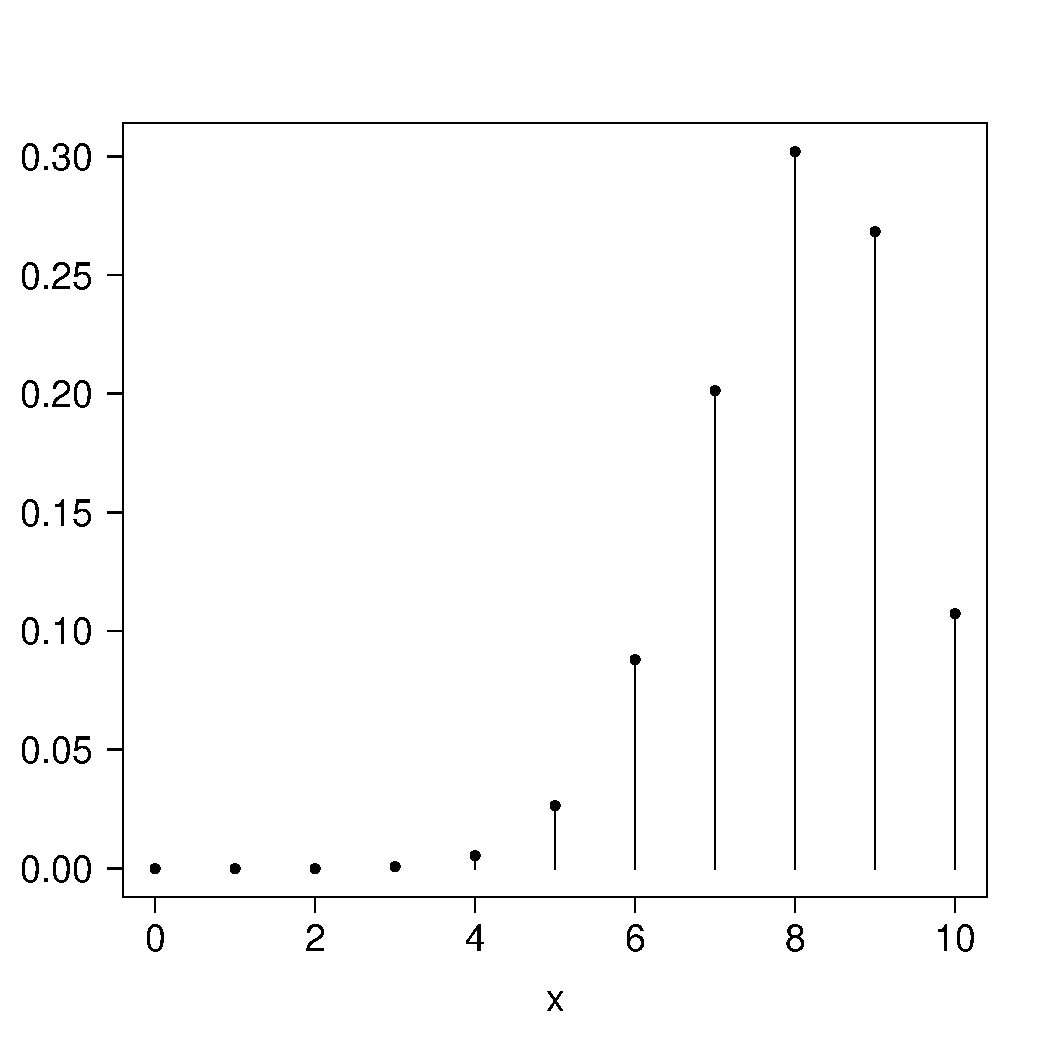
\includegraphics[scale = 0.2]{Binom2.pdf}\\
{\small Binomiale(n=10,p=0.8)}
\end{minipage}
\end{figure}

{\small
Dans tous les cas:
\begin{itemize}
\item Les valeurs possibles sont $0,1,2,\ldots,n$.
\item La valeur de $x$ avec la plus grande probabilité est $np$ (arrondi à l'entier le plus près).
\item La fonction de masse croit jusqu'à $x=np$ puis décroit par la suite.
\end{itemize}
}

\end{frame}

\begin{frame}[t]{Loi binomiale}
Si $X\sim$Binomiale$(n,p)$, alors\\
{\small
\begin{align*}
E(X) = \sum_x x p(x) &= \sum_{x=0}^{n} x {n\choose x}p^x(1-p)^{n-x} \\
&= \sum_{x={\color{red}1}}^{n}  x \frac{n!}{x!(n-x)!}p^x(1-p)^{n-x} \\
&= np \sum_{x=1}^{n}  \frac{(n-1)!}{(x-1)!(n-x)!}p^{x-1}(1-p)^{n-x} \\
&= np \sum_{y=0}^{n-1}  \frac{(n-1)!}{y!(n-1-y)!}p^{y}(1-p)^{n-y-1} \; \; \mbox{ en posant } y=x-1\\
& = np 
\end{align*}
}

\end{frame}

\begin{frame}{Loi binomiale}
    

D'où vient la simplification qui nous permet de passer de l'avant-dernière ligne à la dernière?
\end{frame}

\begin{frame}{Variance}

{\small

On peut calculer $V(X)$ de façon similaire à $E(X)$.\\ 

\vspace{0.2in}
Plus simplement : \alerter{Si $X \sim$ Binomiale$(n,p)$ alors on peut écrire $$X = Y_1, + \hdots + Y_n$$ où les $Y_i$ sont des variables aléatoires de loi Bernoulli(p) indépendantes.}

\begin{align*}
V(X) &= V\left(\sum_{i=1}^n Y_i \right)\\
&= \sum_{i=1}^n V(Y_i) \; \; \mbox{ car } Y_i \perp Y_j, i \ne j \; \; \\
&= \sum_{i=1}^n p(1-p) \; \; \mbox{ car } Y_i \sim \mbox{Bernoulli}(p) \;  \forall p\\
&= np(1-p)
\end{align*}

}


\end{frame}

\section{Loi géométrique}

\begin{frame}[t]{Loi géométrique}
On suppose
\begin{itemize}
 \item une suite d'essais \alerter{indépendants};
 \item chaque essai résulte en un succès ou un échec;
 \item la probabilité de succès à chaque essai est
 $p$;
 \item on arrête l'expérience lorsqu'on obtient \alerter{un premier succès}.
\end{itemize}

\medskip
Soit $X$, le \alerter{nombre total d'essais nécessaires} pour oBoitenir
ce premier succès.

\bigskip
On dit que $X$ suit une loi géométrique avec probabilité de succès $p$, ce qu'on dénote
$$X\sim \mbox{Géométrique} (p).$$
\end{frame}


\begin{frame}{Loi géométrique}

Si $X\sim$Géométrique$(p)$,
\begin{align*}
p(x) = P(X=x) &= P(x-1 \mbox{ échecs suivis de 1 succès}) 
\end{align*}

\vspace{0.1in}
Donc, 
$$p(x)=\left\{\begin{array}{ll}
(1-p)^{x-1}p, & x=1,2,\ldots\\
0, & \text{sinon}.
\end{array}\right.$$

\end{frame}

\begin{frame}{Loi géométrique}
    

Vérifiez que $p(x)$ donnée plus haut est bien une fonction de probabilité de masse. 
\vspace{5cm}

\end{frame}

\begin{frame}{Loi géométrique}

\vspace{-0.1 in}

\begin{figure}[ht]
\begin{minipage}[b]{0.45\linewidth}
\centering
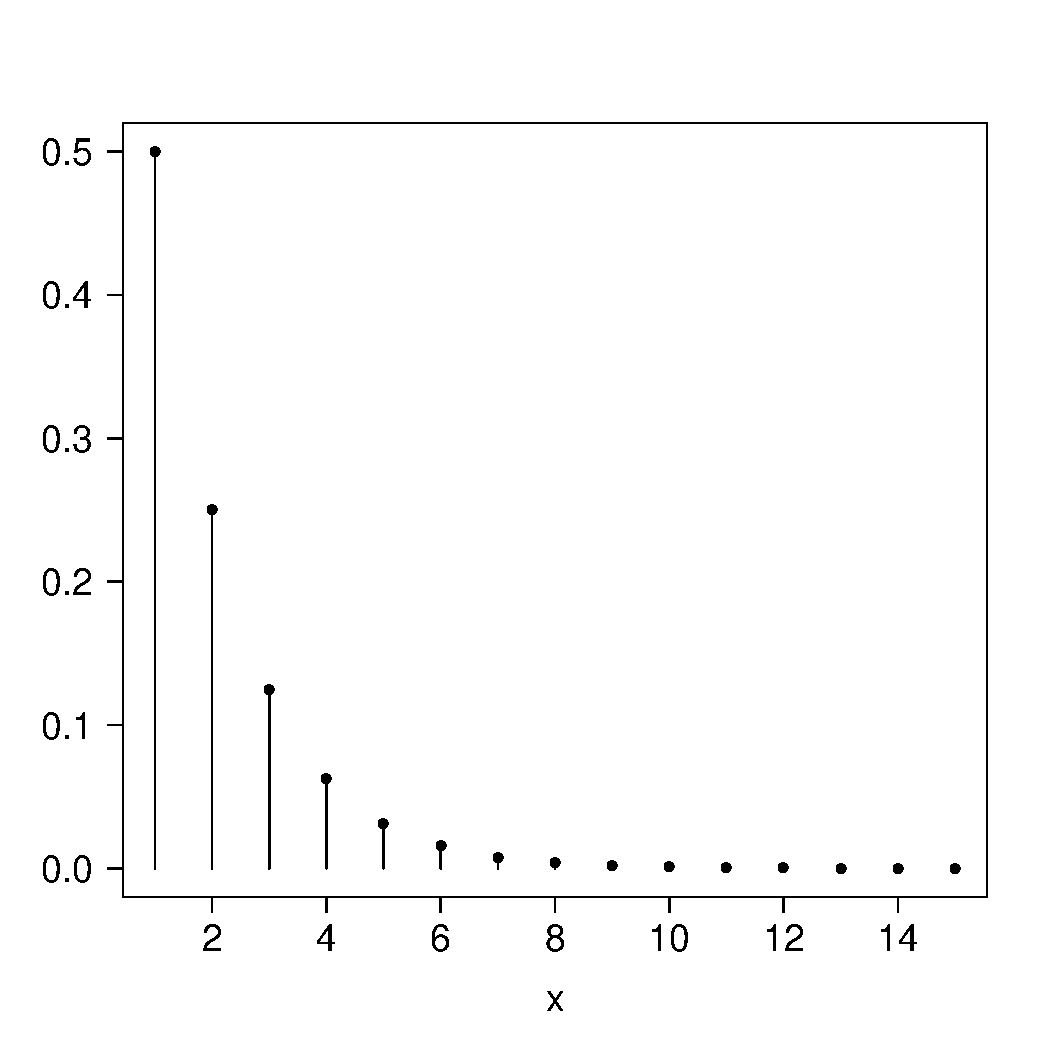
\includegraphics[scale = 0.2]{Geo1.pdf}\\
Géométrique(p=0.5)
\end{minipage}
\hspace{0.5cm}
\begin{minipage}[b]{0.45\linewidth}
\centering
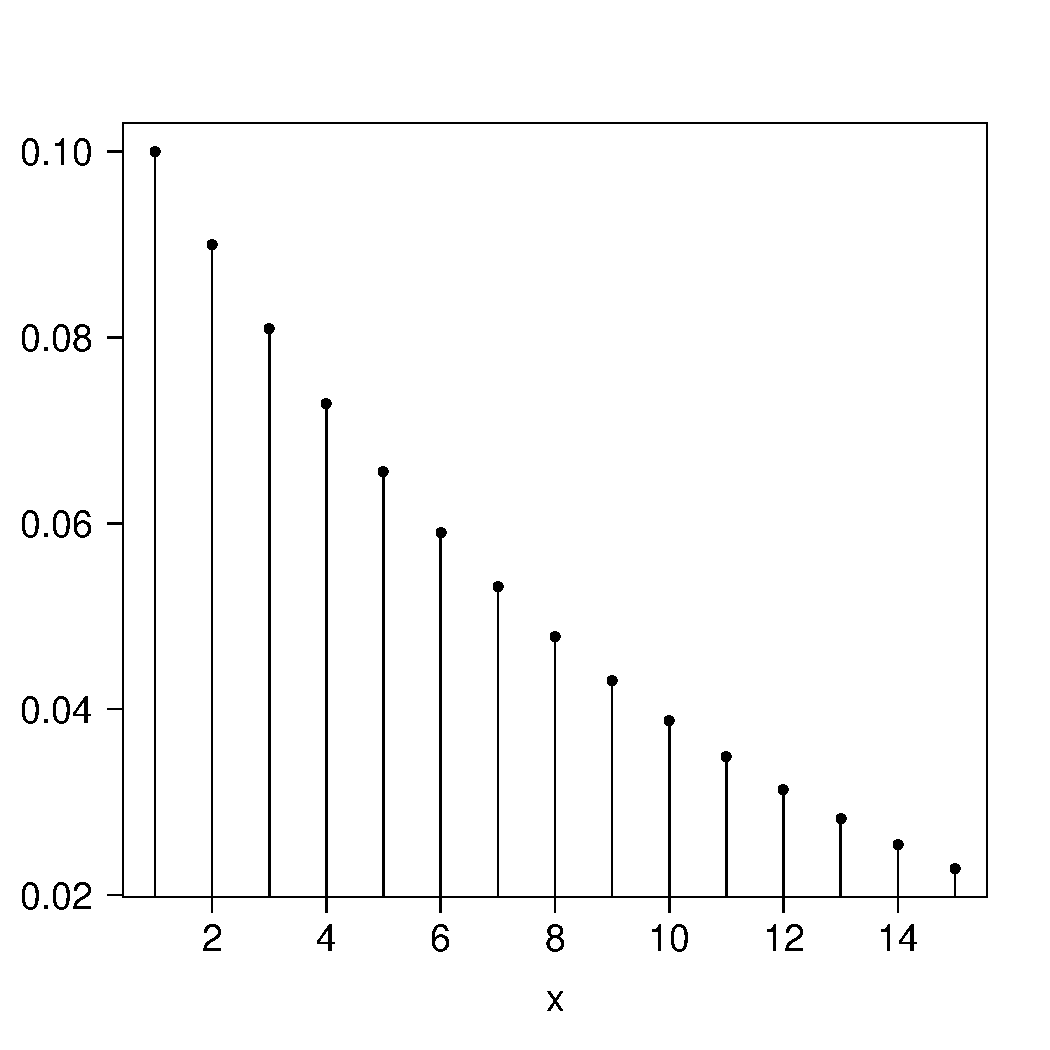
\includegraphics[scale = 0.2]{Geo2.pdf}\\
Géométrique(p=0.1)
\end{minipage}
\end{figure}

{\small
Dans tous les cas:
\begin{itemize}
\item Les valeurs possibles sont tous les entier positifs $(1,2,\ldots,)$.
\item La fonction de masse est décroissante.
\item Plus $p$ est grand, plus elle décroît rapidement.
\end{itemize}
}

\end{frame}

\begin{frame}[t]{Loi géométrique}
Si $X\sim$Géométrique$(p)$, alors

\begin{align*}
    E(X)=1/p & & V(X)=(1-p)/p^2
\end{align*}

{\footnotesize
Preuve pour l'espérance:
\begin{align*} 
E(X) = \sum_{x}^\infty x p(x) &= \sum_{x=1}^\infty x (1-p)^{x-1}p \\
&= \left[ \frac{d}{dp} \sum_{x=1}^\infty (1-p)^x \right] p (-1) \\
&= -p\; \frac{d}{dp} \frac{1-p}{p} \\
&= -p \frac{ (-1)*p - (1-p)*1}{p^2} \\
&= \frac{1}{p}
\end{align*} 
}
\end{frame}


\begin{frame}{Propriété intéressante}
La loi géométrique est \alerter{la seule loi discrète \underline{sans mémoire}}, c'est-à-dire que
\alerter{$$P[X>x+s|X>s]=P[X>x]$$}
pour tous $x,s=1,2,3,\ldots$.


\vspace{0.2in}
En d'autres mots, le nombre d'essais pour oBoitenir un succès ne dépend pas du nombre d'essais déjà effectués.

\end{frame}

\section{Loi binomiale négative (Pascal)}

\begin{frame}[t]{Loi binomiale négative (Pascal)}
On suppose
\begin{itemize}
 \item une suite d'essais \alerter{indépendants};
 \item chaque essai résulte en un succès ou un échec;
 \item la probabilité de succès \alerter{à chaque essai} est
 $p$;
 \item on arrête l'expérience lorsqu'on obtient \alerter{un $r$-ème succès}.
\end{itemize}

\medskip
Soit $X$, le \alerter{nombre total d'essais nécessaires} pour oBoitenir
ces $r$ succès.

\bigskip
On dit que $X$ suit une loi négative binomiale avec paramètres $r$ et $p$, ce qu'on dénote
$$X\sim \text{NB}(r,p).$$

À noter, le livre utilise le terme "loi de Pascal", ce qui est peu utilisé en pratique.
\end{frame}

\begin{frame}{Loi binomiale négative}

Si $X\sim\text{NB}(r,p)$,
\begin{align*}
p(x) = P(X=x) &= P(x \mbox{essais avant d'avoir $r$ succès}) 
\end{align*}

Donc, 
\begin{itemize}
\item On doit oBoitenir $r$ succès et $x-r$ échecs.
\item Le dernier essai doit être un succès. 
\item Les autres $r-1$ succès peuvent être positionnés de n'importe quelle façon dans les premiers $x-1$ essais. 
\end{itemize}


\vspace{0.1in}
Donc, 
$$p(x)=\left\{\begin{array}{ll}
{x-1\choose r-1}p^r(1-p)^{x-r}, & x=r,r+1,\ldots\\
0, & \text{sinon}.
\end{array}\right.$$

\end{frame}

\begin{frame}{Loi binomiale négative}

\vspace{-0.1 in}

\begin{figure}[ht]
\begin{minipage}[b]{0.45\linewidth}
\centering
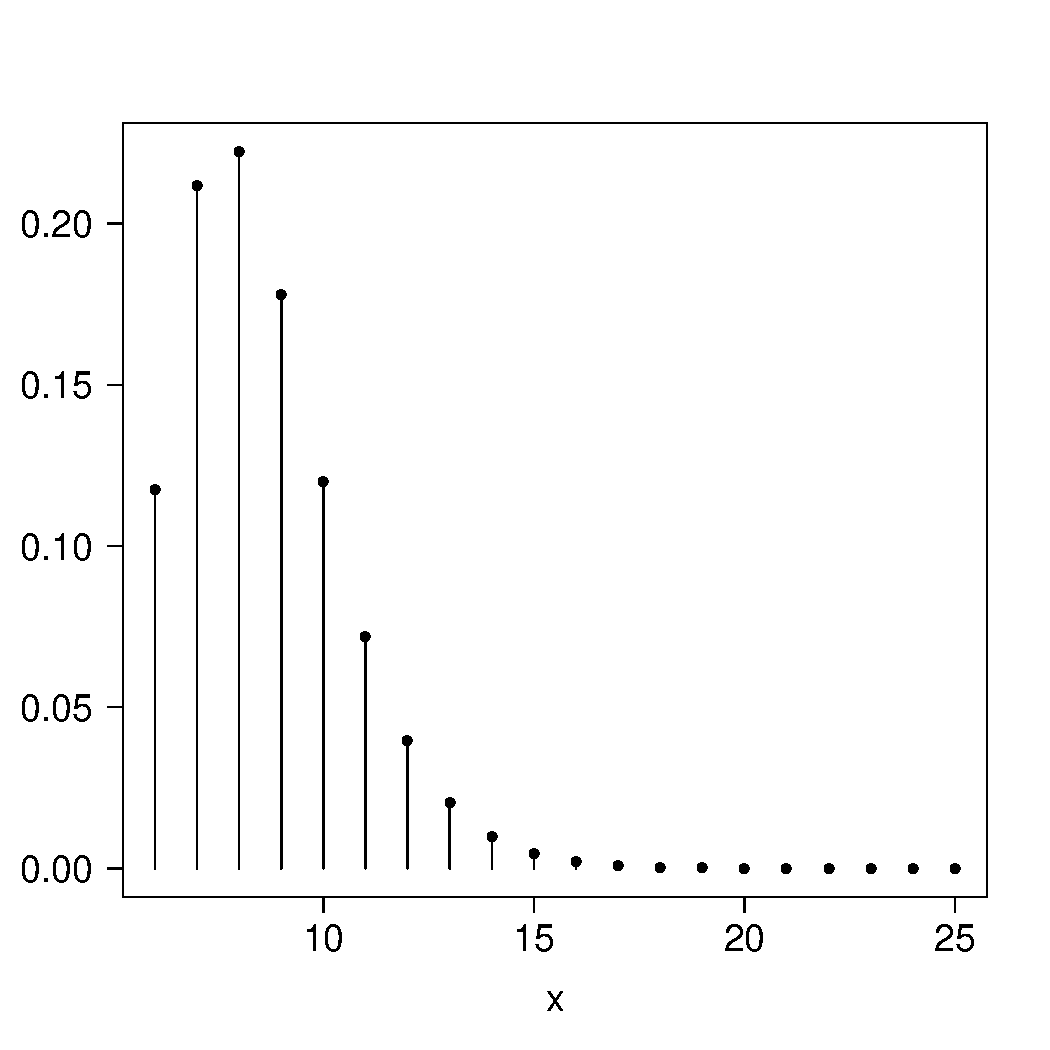
\includegraphics[scale = 0.2]{Pascal2.pdf}\\
Pascal(r=6,p=0.7)
\end{minipage}
\hspace{0.5cm}
\begin{minipage}[b]{0.45\linewidth}
\centering
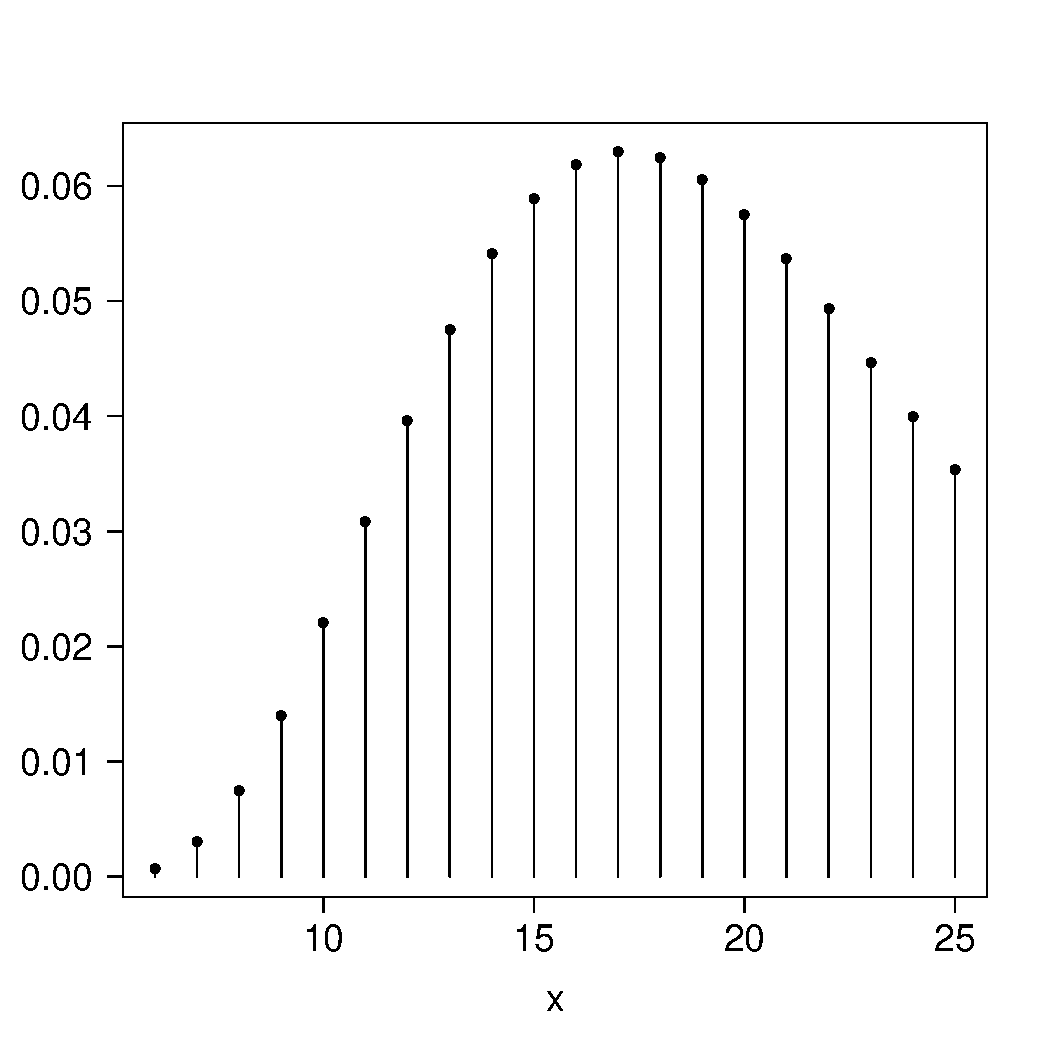
\includegraphics[scale = 0.2]{Pascal1.pdf}\\
Pascal(r=6,p=0.3)
\end{minipage}
\end{figure}

{\small
Dans tous les cas:
\begin{itemize}
\item Les valeurs possibles sont tous les entiers positifs plus grands que $r$ ($r,r+1,\ldots)$.
\item Plus $p$ est petit, plus les valeurs probables sont grandes.
\item Plus $r$ est grand, plus les valeurs probables sont grandes.
\end{itemize}
}

\end{frame}

\begin{frame}[t]{Espérance et variance}

\alerter{Si $X \sim \mbox{NB}(r,p)$, alors on peut écrire
$$ X = Y_1 + \hdots + Y_r$$
 o\`u les $Y_i$ sont indépendantes et $Y_i \sim \mbox{Géométrique}(p)$ pour tout $ i$.}
\vspace{0.1 in}

Donc, 
$$E(X) = \frac{r}{p}$$
et
$$V(X) = r\frac{(1-p)}{p^2}$$

\end{frame}

\section{Loi de Poisson}

\begin{frame}[t]{Loi de Poisson}

{\small
On obtient habituellement une loi de Poisson dans l'une des
deux situations suivantes:
\begin{itemize}
\item {\bf Loi des événements rares:} Considérons $X$ une
v.a. binomiale o\`u $n$ est très, très grand et $p$
est très, très petit. Soit $\mu$ la limite de $np$ quand
$n\to\infty$ et $p\to0$. Alors on peut montrer qu'à la limite,
on obtient
$$p(x)=\left\{\begin{array}{ll}
\frac{\mu^x e^{-\mu}}{x!}, & x=0,1,2,\ldots,\\
0, & \text{sinon}.\end{array}\right.$$
\item {\bf Nombre d'événements dans un intervalle de temps fixé
({\it Processus de Poisson}):}
Sous certaines conditions, si on observe en moyenne $\lambda$
événements par unité de temps (ou d'espace), alors le
nombre d'événements $X$ dans $t$ unités de temps (ou d'espace) suit
une loi de Poisson de moyenne $\mu=\lambda t$. \\
(On y reviendra au module 4.)
\end{itemize}
}
\end{frame}

\begin{frame}{Loi de Poisson}
Si $X\sim$Poisson$(\mu)$, alors
$$p(x)=\left\{\begin{array}{ll}
\frac{\mu^x e^{-\mu}}{x!}, & x=0,1,2,\ldots,\\
0, & \text{sinon}.\end{array}\right.$$

\vspace{0.2in}
Si $X\sim$Poisson$(\mu)$, alors
$$E(X)=\mu$$
$$V(X)=\mu$$

\vspace{0.2in}
Voir les preuves à la page 125 du manuel. 
\end{frame}

\begin{frame}{Loi de Poisson}

\vspace{-0.1 in}

\begin{figure}[ht]
\begin{minipage}[b]{0.45\linewidth}
\centering
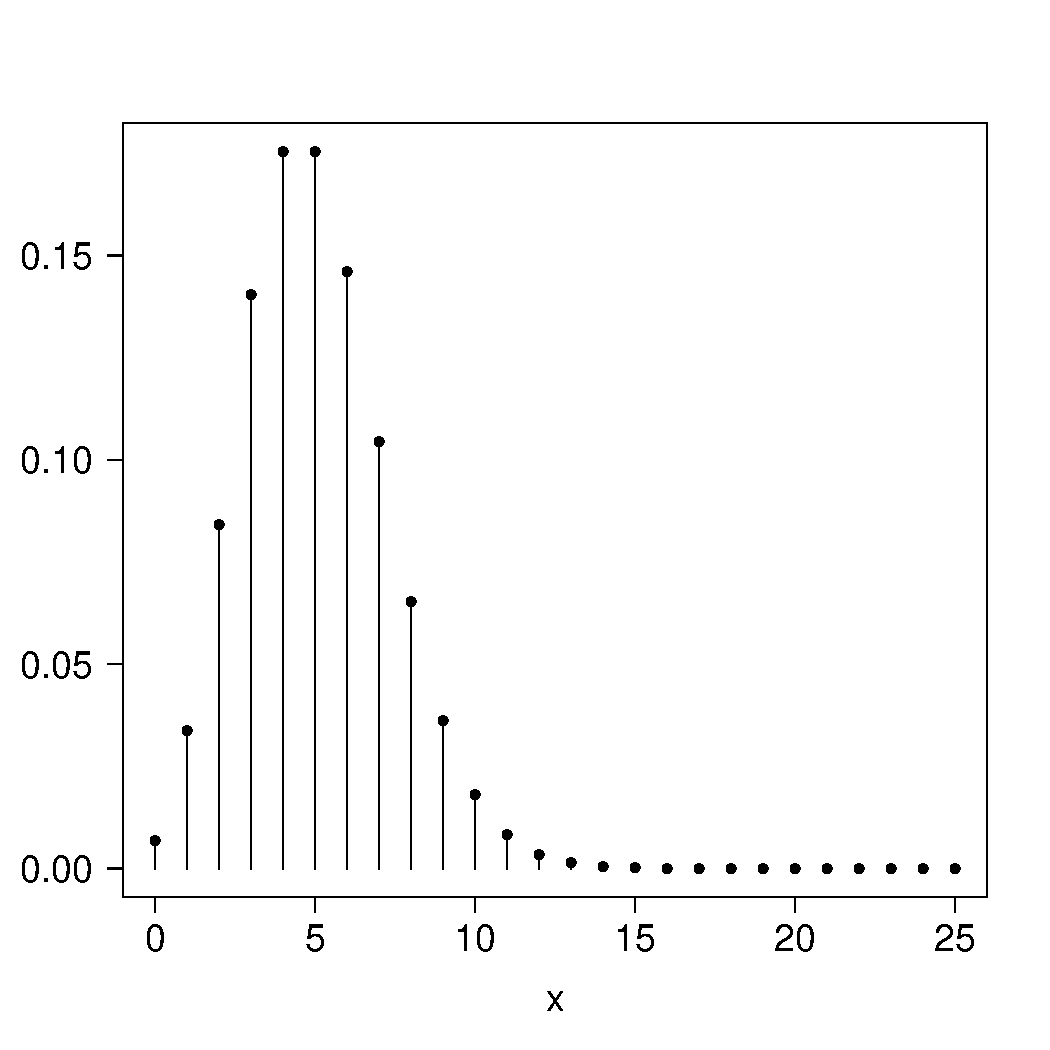
\includegraphics[scale = 0.2]{Poisson1.pdf}\\
Poisson($\mu=5$)
\end{minipage}
\hspace{0.5cm}
\begin{minipage}[b]{0.45\linewidth}
\centering
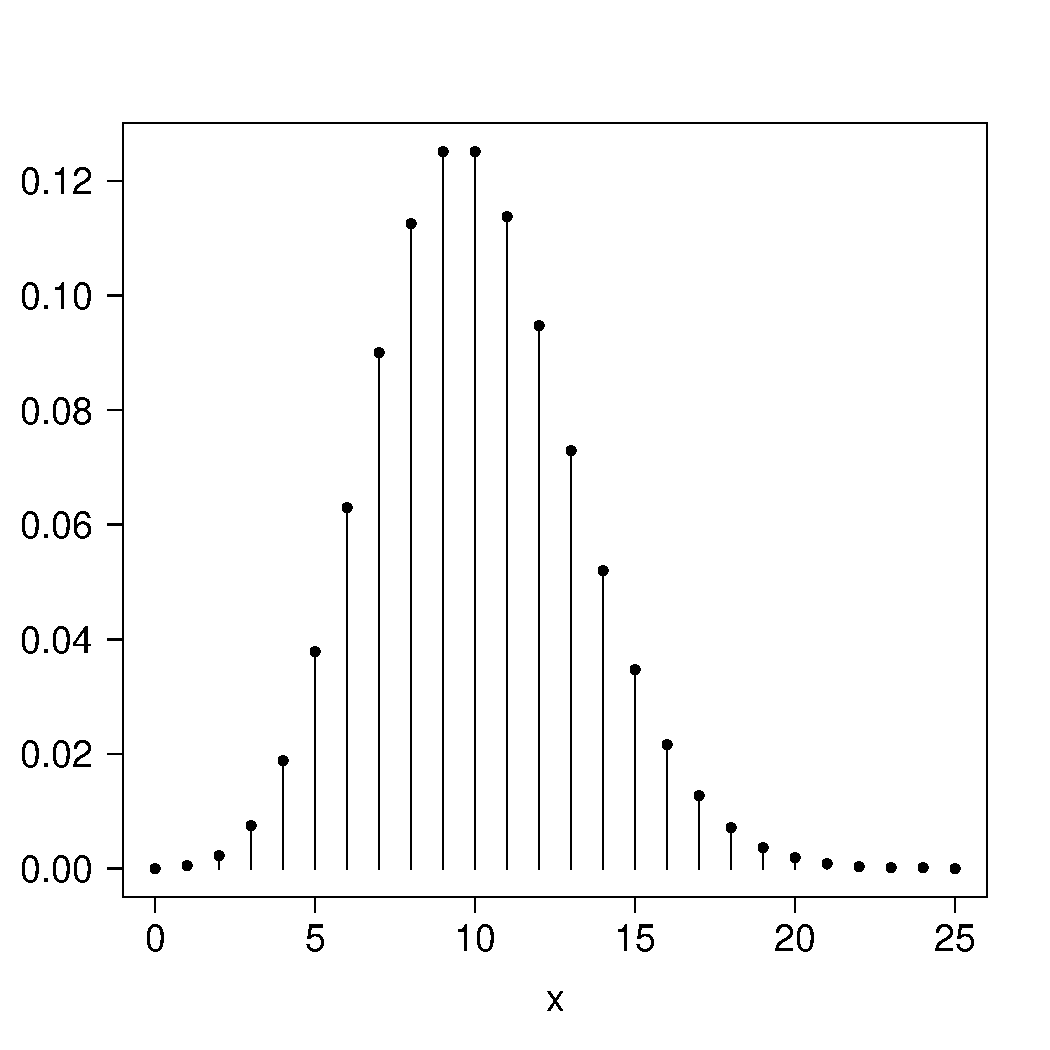
\includegraphics[scale = 0.2]{Poisson2.pdf}\\
Poisson($\mu=10$)
\end{minipage}
\end{figure}

{\small
Dans tous les cas:
\begin{itemize}
\item Les valeurs possibles sont tous les entier non-négatifs ($0,1,2,\ldots)$.
\item Les valeurs les plus probables sont concentrées autour de l'espérance.
\end{itemize}
}

\end{frame}

\begin{frame}{Loi de Poisson}

La loi de Poisson a deux propriétés importantes:
\vspace{0.1in}

\textbf{Additivité:}\\
Si $X_1,\hdots,X_n$ sont des v.a. indépendantes avec $X_i\sim$Poisson$(\mu_i)$ et
$Y=X_1+\hdots+X_n$, alors

$$Y\sim \mbox{ Poisson}(\mu_1+\cdots+\mu_n).$$


\vspace{0.1in}
\textbf{Approximation de la binomiale:}\\
Lorsque $n$ est grand et $p$ est petit, on peut approximer la loi Binomiale$(n,p)$ par une loi Poisson($\mu=np$).

\end{frame}

\section{Quelques exemples}

\begin{frame}[t]{Tirs d'un chasseur}

{\small
Un chasseur a une chance sur 3 d'atteindre une cible à chaque balle
qu'il tire, et ses résultats d'un tir à l'autre sont indépendants.
Quelle est la probabilité qu'il lui faudra tirer 4, 5 ou 6 balles
pour atteindre sa cible? 
}


\end{frame}


\begin{frame}[t]{Tirs d'un chasseur (suite)}

{\small
Combien de balles seront requises en moyenne pour atteindre la cible?
}


\vspace{1in}
{\small
Combien de balles, en moyenne, sont requises pour que ce
chasseur atteigne 5 cibles? 
}
\end{frame}


\begin{frame}[t]{Tirs d'un chasseur (suite)}

{\small
Quelle est la probabilité que plus de 6 balles soient requises pour atteindre 5 cibles?
}



\end{frame}


\begin{frame}[t]{Examen à choix multiples}

{\small Un examen compte 20 questions à choix multiples, avec 5 choix
de réponses à chacune des questions. Si on répond de façon
complètement aléatoire aux 20 questions et que l'on reçoit
10 points pour une bonne réponse et -2 points pour une mauvaise
réponse, quel est notre score attendu à cet examen?
}

\end{frame}

\begin{frame}[t]{Des bulles d'air dans le béton}

%Changer éventuellement

{\small
Le nombre de bulles d'air dans un mélange de béton suit une loi
de Poisson de moyenne 1 bulle par $10~m^3$. Quelle est la probabilité
qu'un pavé fait avec $20~m^3$ de ce béton ait au moins
une bulle d'air?

\vspace{1.5in}
  Quelle est la moyenne du nombre de bulles
dans de tels pavés?
}
\end{frame}


\begin{frame}[t]{Calcul de revenus}

{\small
Une firme d'informaticiens est engagée pour concevoir un logiciel de prise en rendez-vous . Elle sera payée $25~000\$$ pour ce travail, plus un bonus de $5~ 000\$$ si le logiciel est terminé à la date prévue. Quelle est la moyenne et la variance des revenus de cette compagnie pour ce contrat si la probabilité de terminer dans les temps est de $20\%$?

%\uncover<2->{
%\vspace{0.1 in}
%On définit 2 v.a.:\\
%$X = 1$ si la construction est terminée à temps, et 0 sinon. \\
%$Y=$ revenus pour la construction de l'hôpital.
%}
%
%\uncover<3->{
%\vspace{0.1in}
%D'après la mise en situation, 
%$$X \sim \mbox{Bernoulli}(0.2) \mbox{ et } Y = 25000 + 5000X.$$
%}
%
%\vspace{-0.1 in}
%\uncover<4->{
%$X \sim \mbox{Bernoulli}(0.2) \implies E(X) = 0.2$ et $V(X) = 0.2*0.8 = 0.16$. 
%\vspace{0.05 in}
%}
%
%\uncover<5->{
%Donc, \\
%$E(Y) = E(25000 + 5000X) = 25000 + 5000*E(X) = 26\;000 \$.$\\}
%\uncover<6->{
%$V(X) = V(25000 + 5000X) = 5000^2 V(X) = 4\;000\;000 \$^2 $
%}

}

\end{frame}

\begin{frame}[t]{Lancers d'une pièce de monnaie}

{\small 

On lance une pièce de monnaie balancée 10 fois. On suppose que les résultats oBoitenus à chaque lancer sont
indépendants. Calculez
\begin{enumerate}
 \item[(i)] l'espérance et la variance du nombre de ``pile'' oBoitenus;
 \item[(ii)] la probabilité d'oBoitenir exactement deux ``pile'';
 \item[(iii)] la probabilité d'oBoitenir au moins deux ``pile''.
\end{enumerate}
}
%\vspace{0.05 in}
%\uncover<2->{
%Soit X le nombre de ``pile'' oBoitenus en 10 lancers. \\
%Alors, $X \sim$ Binomiale$(10,0.5)$. 
%}
%\begin{enumerate}
%\uncover<3->{
%\item[(i)] $E(X) = np = 10*0.5 = 5$\\
%$V(X) = np(1-p) = 10*0.5*0.5 = 2.5$}
%\uncover<4->{
%\item[(ii)]
%$P(X=2) = {10 \choose 2} 0.5^2 (1-0.5)^8 = 0.0439$}
%\uncover<5->{
%\item[(iii)]
%$P(X > 2) = 1-P(X\le 2)$, donc
%\begin{align*}
%P(X > 2) &= 1-(P(X=0) + P(X=1))\\
%&= 1 - {10 \choose 0} 0.5^0 (1-0.5)^10 - {10 \choose 1} 0.5^1 (1-0.5)^9 \\
%&= 0.9892578
%\end{align*}
%}
%\end{enumerate}
%


\end{frame}


\begin{frame}[t]{Des entrevues}

{\small
 Une entreprise doit faire passer des entrevues jusqu'à
 l'embauche de 2 nouveaux employés. Chaque entrevue résulte en une
 embauche avec probabilité de 25\% et les décisions prise à
 chacune des entrevues sont indépendantes. Une entrevue résultant
 en une embauche co\^ute 500\$ et une entrevue ne résultant pas
 en une embauche co\^ute 100\$. Quels sont l'espérance et
 l'écart-type du co\^ut total des entrevues?
}
%
%\vspace{0.1 in}
%\uncover<2->{Soit $X$ le nombre d'entrevues et $Y$ le coût total des entrevues \\
%Alors, 
%$$X \sim \mbox{ Pascal}(2,0.25)$$ 
%$$Y = 2*500 + (X-2)*100 = 800 + 100X$$
%}
%
%\uncover<3->{Donc, \\
%\begin{itemize}
%\item $E(Y) = 800 + 100E(X) = 800 + 100 \frac{2}{0.25} = 1600 \$$}
%\uncover<4->{
%\item $V(X) = V(800 + 100X) = 100^2V(X) = 100^2 \frac{2(1-0.25)}{0.25^2} = 240 000 \$^2$
%$\implies \sigma_Y = \sqrt{V(Y)} \approx 489.9 \$$}
%\end{itemize}

\end{frame}



\begin{frame}{Bibliographie}
 	Ce document est rédigé avec Beamer ainsi qu'une classe .cls fourni par Jérôme Soucy. Les diapositives sont adaptées des diapositives créées par Anne-Sophie Charest 
 pour le cours STT-1000. Les graphiques proviennent de ces mêmes diapositives.
 	\printbibliography
 	\vfill
 	\footnotesize Pour signaler une erreur dans ce document, veuillez écrire à l'adresse :~\href{mailto:julien.miron@mat.ulaval.ca}{julien.miron@mat.ulaval.ca}.
 \end{frame}

\end{document}

